\documentclass[12pt]{article}

% TEMPLATE DEFAULT PACKAGES
\usepackage{amssymb,amsmath,amsfonts,eurosym,geometry,ulem,graphicx,color,setspace,sectsty,comment,natbib,pdflscape,array,adjustbox}

% ADDED PACKAGES FOR THIS MANUSCRIPT
\usepackage{palatino,newtxmath,multirow,titlesec,threeparttable,tabu,booktabs,titlesec,threeparttable,mathtools,bm,bbm,subcaption,pdflscape,tcolorbox,mathrsfs}
% endfloat,

\usepackage{afterpage}
\usepackage[hyphens]{url}
\usepackage[margin=1cm]{caption}

\usepackage[draft]{hyperref}
\newcommand{\tim}{$\,\times\,$}
% FIGURES & TABLES CAPTION STYLING
\captionsetup[figure]{labelfont={bf},name={Figure},labelsep=period}
\captionsetup[table]{labelfont={bf},name={Table},labelsep=period}

% SECTION TITLE SETTINGS
\titlelabel{\thetitle.\enskip}
\titleformat*{\section}{\large\bfseries}
\titleformat*{\subsection}{\normalsize\bfseries}

% COLUMN TYPES
\newcolumntype{L}[1]{>{\raggedright\let\newline\\\arraybackslash\hspace{0pt}}m{#1}}
\newcolumntype{C}{>{\centering\arraybackslash}p{5.2em}}
\newcolumntype{D}{>{\centering\arraybackslash}p{5em}}
\newcolumntype{R}[1]{>{\raggedleft\let\newline\\\arraybackslash\hspace{0pt}}m{#1}}


% MARGINS AND SPACING
\normalem
\geometry{left=1.1in,right=1.1in,top=1.0in,bottom=1.0in}
\setlength{\parskip}{2.5pt}

% SPECIAL CELL 
\newcommand{\specialcell}[2][c]{%
	\begin{tabular}[#1]{@{}l@{}}#2\end{tabular}}

% NO INDENT ON FOOTNOTES
\usepackage[hang,flushmargin]{footmisc}

\begin{document}



\vspace{0mm}
\begin{table}[h!]
\centering
\caption{Housing Project Areas Description}\label{table:projectdescriptives}
\vspace{0mm}
\begin{tabular}{l*{1}{cccccc}}
\toprule
  & \multicolumn{2}{c}{\textbf{All}}& \multicolumn{2}{c}{\textbf{Greenfield}}  & \multicolumn{2}{c}{\textbf{In-Situ}}   \\
  &Const. & Unconst. &Const. & Unconst.   & Const. & Unconst. \\
\midrule
 Number of Projects  & 172  & 145  & 43  & 20  & 27  & 29  \\ 
 Area (km2)  & 1.17  & 1.16  & 1.72  & 2.42  & 1.50  & 0.88  \\ 
 Median Construction Yr.  & 2006  & 2006  & 2006  & 2005  & 2004  & 2006  \\ 
 Delivered Houses  & 374  & 11  & 568  & 24  & 702  & 20  \\ 
 House Price in 1 km (R$^\dagger$)  & 188,441  & 218,635  & 194,214  & 186,841  & 179,596  & 208,570  \\ 
 Distance to CBD$^\ddagger$ (km)  & 32.5  & 27.7  & 40.5  & 39.9  & 32.6  & 30.6  \\ 

\bottomrule
\multicolumn{7}{l}{\scriptsize Const. refers to constructed projects and unconst. refers to unconstructed projects.}\\[-.5em]
\multicolumn{7}{l}{\scriptsize $^*$Calculated from {\it expected} completion dates using Gauteng National Treasury budget reports.}\\[-.5em]
\multicolumn{7}{l}{\scriptsize $^\dagger$ The USD averaged to about 7.70 Rands during the 2001-2011 period.}\\[-.5em]
\multicolumn{7}{l}{\scriptsize $^\ddagger$Measured as the average minimum distance with respect to Johannesburg and Pretoria CBDs. } \\[-.5em]
%\multicolumn{7}{l}{\scriptsize City includes projects whose centroids are within 30.4 km of their nearest CBD.} \\[-.5em]
%\multicolumn{7}{l}{\scriptsize Suburb includes projects whose centroids are further than 30.4 km from their nearest CBD.}
\end{tabular}
\end{table} 



\begin{figure*}
        \centering
   %     \caption[ Pre-Period Housing Densities in Constructed and Unconstructed Projects Areas ]
  %      {\small Pre-Period Densities} 
        %\vspace{2mm}
        \begin{subfigure}[b]{0.48\textwidth}
                    \caption[Network2]%
            {{\footnotesize \textbf{All Projects} pre-period formal raw data}}    
            \label{fig:prefor}
            \centering
            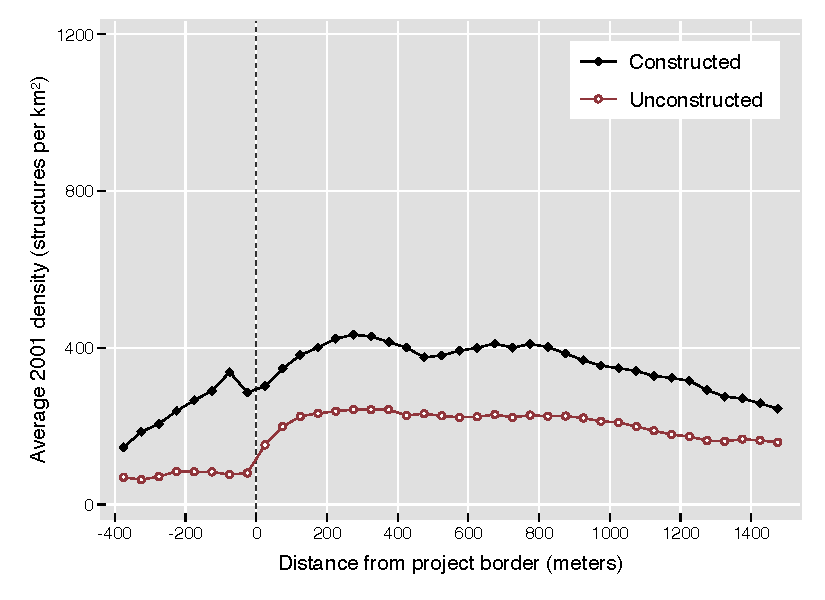
\includegraphics[width=\textwidth,trim={0.3cm .3cm 0.1cm 0cm}, clip=true]{figures/bblu_for_pre_means_4_30k.pdf}

        \end{subfigure}
        \hfill
        \begin{subfigure}[b]{0.48\textwidth}  
                    \caption[]%
            {{\footnotesize \textbf{All Projects} pre-period informal  raw data}}      
            \label{fig:preinf}
            \centering 
            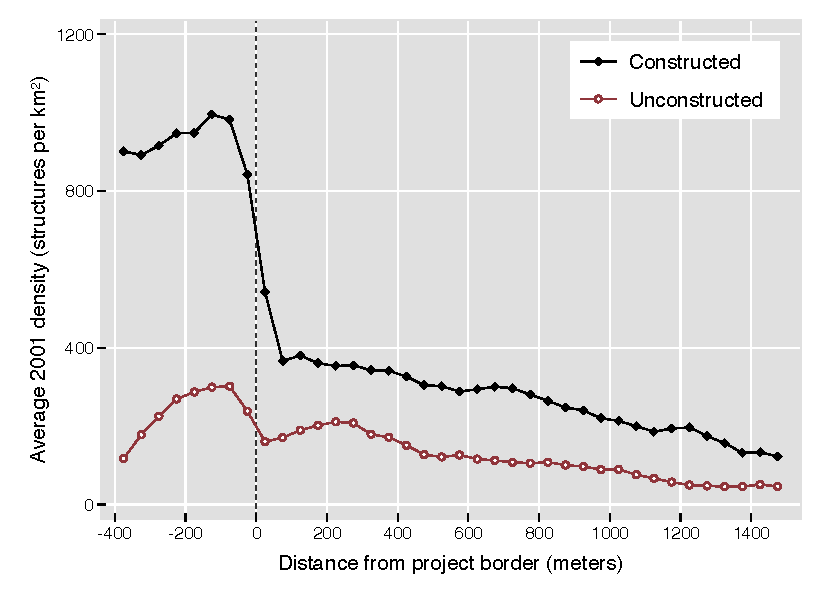
\includegraphics[width=\textwidth,trim={0.3cm .3cm 0.1cm 0cm}, clip=true]{figures/bblu_inf_pre_means_4_30k.pdf}

        \end{subfigure}
        \begin{subfigure}[b]{0.48\textwidth}
                    \caption[Network2]%
            {{\footnotesize \textbf{Greenfield} pre-period formal  raw data}}    
            \label{fig:prefor}
            \centering
            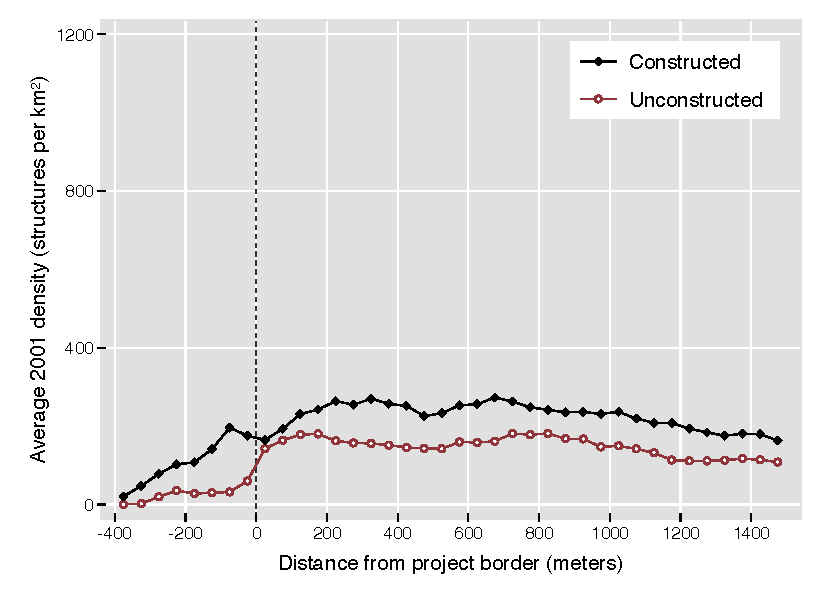
\includegraphics[width=\textwidth,trim={0.3cm .3cm 0.1cm 0cm}, clip=true]{figures/bblu_for_pre_means_4_1_30k.pdf}

        \end{subfigure}
        \hfill
        \begin{subfigure}[b]{0.48\textwidth}  
                    \caption[]%
            {{\footnotesize \textbf{Greenfield} pre-period informal  raw data}}     
            \label{fig:preinf}
            \centering 
            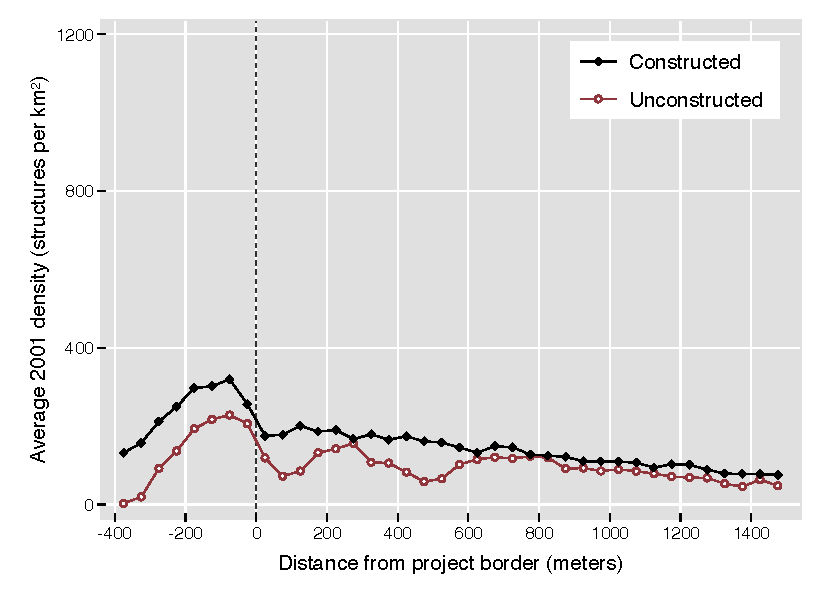
\includegraphics[width=\textwidth,trim={0.3cm .3cm 0.1cm 0cm}, clip=true]{figures/bblu_inf_pre_means_4_1_30k.pdf}

        \end{subfigure}
        \begin{subfigure}[b]{0.48\textwidth}
                    \caption[Network2]%
            {{\footnotesize \textbf{In-Situ} pre-period formal  raw data}}   
            \label{fig:prefor}
            \centering
            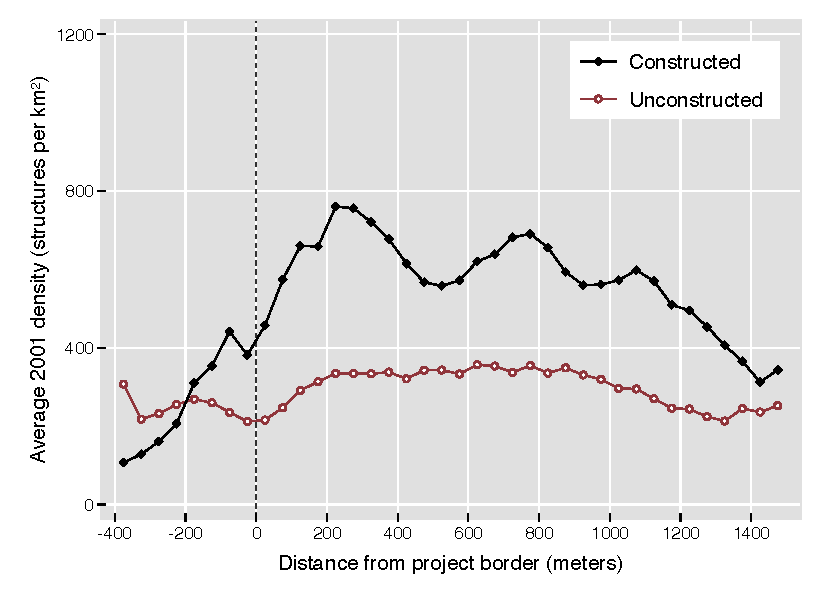
\includegraphics[width=\textwidth,trim={0.3cm .3cm 0.1cm 0cm}, clip=true]{figures/bblu_for_pre_means_4_2_30k.pdf}

        \end{subfigure}
        \hfill
        \begin{subfigure}[b]{0.48\textwidth}  
                    \caption[]%
            {{\footnotesize \textbf{In-Situ} pre-period informal  raw data}}     
            \label{fig:preinf}
            \centering 
            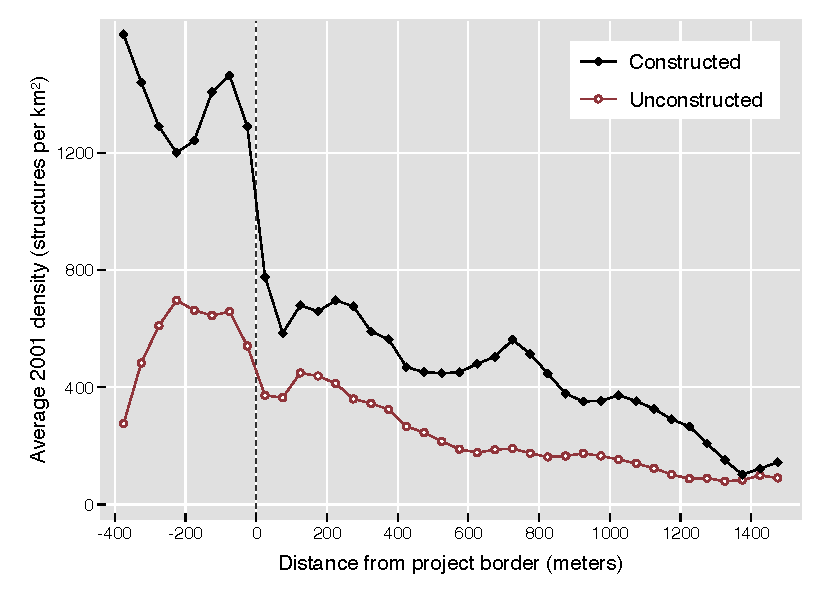
\includegraphics[width=\textwidth,trim={0.3cm .3cm 0.1cm 0cm}, clip=true]{figures/bblu_inf_pre_means_4_2_30k.pdf}

        \end{subfigure}
        \begin{subfigure}[b]{0.48\textwidth}
                    \caption[Network2]%
            {{\footnotesize \textbf{Other} pre-period formal  raw data}}   
            \label{fig:prefor}
            \centering
            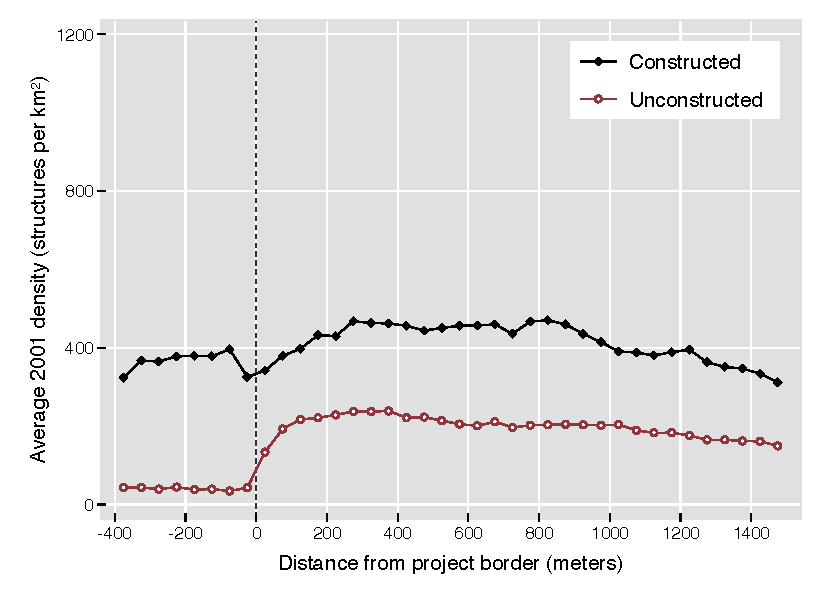
\includegraphics[width=\textwidth,trim={0.3cm .3cm 0.1cm 0cm}, clip=true]{figures/bblu_for_pre_means_4_3_30k.pdf}

        \end{subfigure}
        \hfill
        \begin{subfigure}[b]{0.48\textwidth}  
                    \caption[]%
            {{\footnotesize \textbf{Other} pre-period informal  raw data}}      
            \label{fig:preinf}
            \centering 
            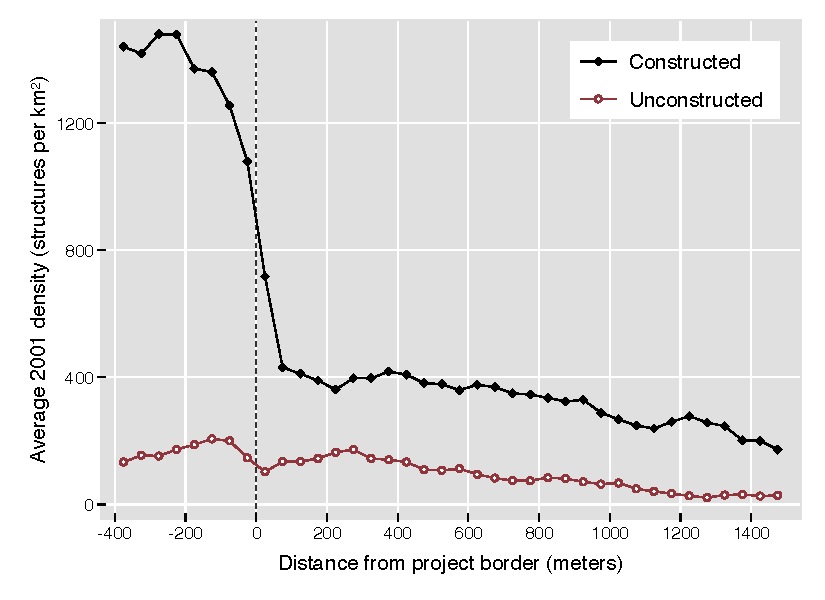
\includegraphics[width=\textwidth,trim={0.3cm .3cm 0.1cm 0cm}, clip=true]{figures/bblu_inf_pre_means_4_3_30k.pdf}

        \end{subfigure}
\end{figure*}


\begin{figure*}
        \centering
   %     \caption[ Pre-Period Housing Densities in Constructed and Unconstructed Projects Areas ]
  %      {\small Pre-Period Densities} 
        %\vspace{2mm}
        \begin{subfigure}[b]{0.48\textwidth}
                    \caption[Network2]%
            {{\footnotesize \textbf{All Projects} pre-period formal lat-lon fe}}    
            \label{fig:prefor}
            \centering
            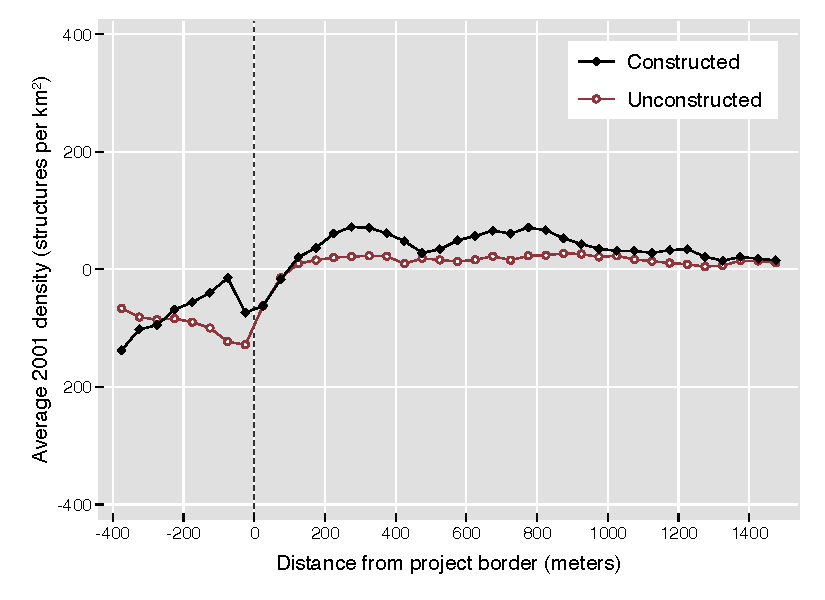
\includegraphics[width=\textwidth,trim={0.3cm .3cm 0.1cm 0cm}, clip=true]{figures/bblu_for_fe_pre_means_4_30k.pdf}

        \end{subfigure}
        \hfill
        \begin{subfigure}[b]{0.48\textwidth}  
                    \caption[]%
            {{\footnotesize \textbf{All Projects} pre-period informal lat-lon fe }}      
            \label{fig:preinf}
            \centering 
            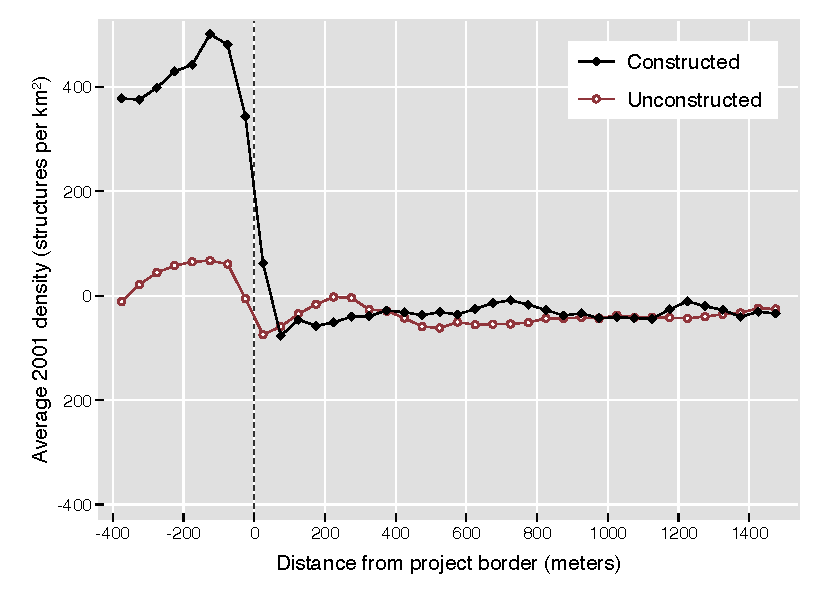
\includegraphics[width=\textwidth,trim={0.3cm .3cm 0.1cm 0cm}, clip=true]{figures/bblu_inf_fe_pre_means_4_30k.pdf}

        \end{subfigure}
        \begin{subfigure}[b]{0.48\textwidth}
                    \caption[Network2]%
            {{\footnotesize \textbf{Greenfield} pre-period formal lat-lon fe }}    
            \label{fig:prefor}
            \centering
            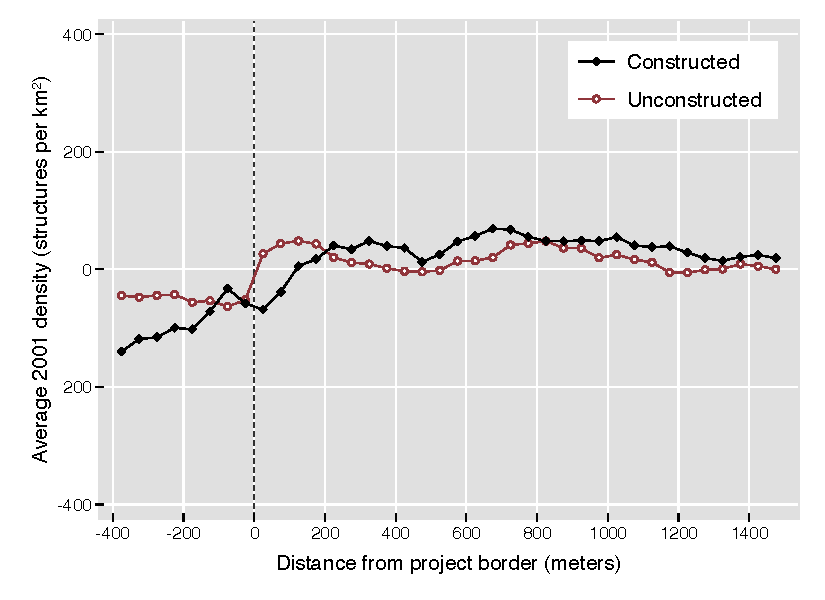
\includegraphics[width=\textwidth,trim={0.3cm .3cm 0.1cm 0cm}, clip=true]{figures/bblu_for_fe_pre_means_4_1_30k.pdf}

        \end{subfigure}
        \hfill
        \begin{subfigure}[b]{0.48\textwidth}  
                    \caption[]%
            {{\footnotesize \textbf{Greenfield} pre-period informal lat-lon fe }}     
            \label{fig:preinf}
            \centering 
            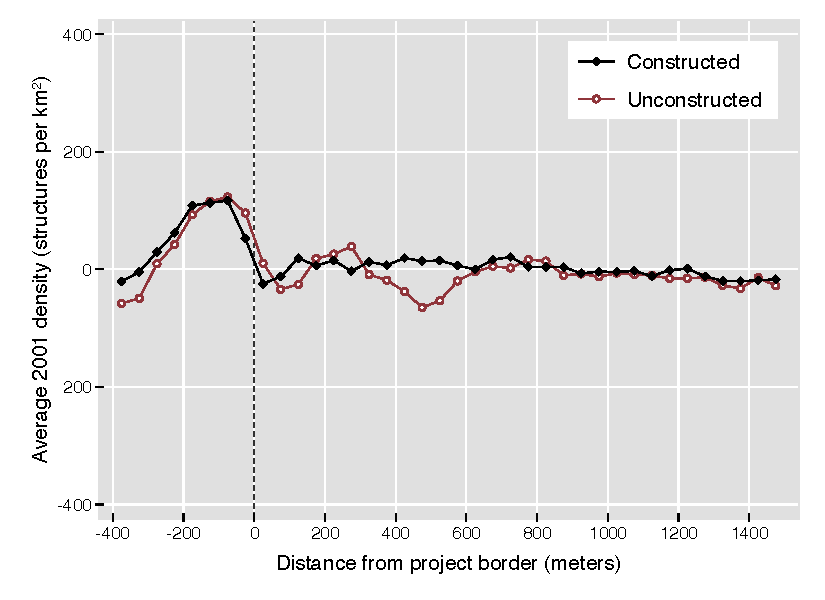
\includegraphics[width=\textwidth,trim={0.3cm .3cm 0.1cm 0cm}, clip=true]{figures/bblu_inf_fe_pre_means_4_1_30k.pdf}

        \end{subfigure}
        \begin{subfigure}[b]{0.48\textwidth}
                    \caption[Network2]%
            {{\footnotesize \textbf{In-Situ} pre-period formal lat-lon fe }}   
            \label{fig:prefor}
            \centering
            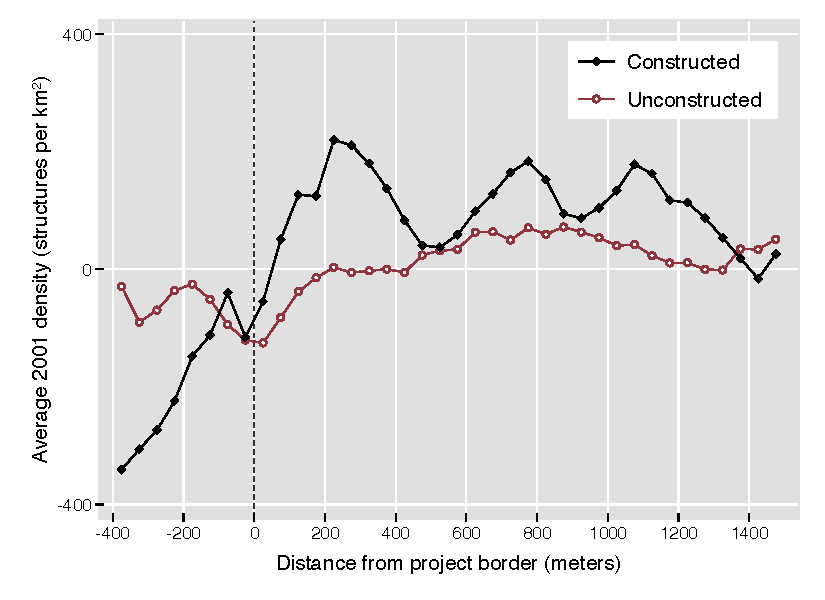
\includegraphics[width=\textwidth,trim={0.3cm .3cm 0.1cm 0cm}, clip=true]{figures/bblu_for_fe_pre_means_4_2_30k.pdf}

        \end{subfigure}
        \hfill
        \begin{subfigure}[b]{0.48\textwidth}  
                    \caption[]%
            {{\footnotesize \textbf{In-Situ} pre-period informal lat-lon fe }}     
            \label{fig:preinf}
            \centering 
            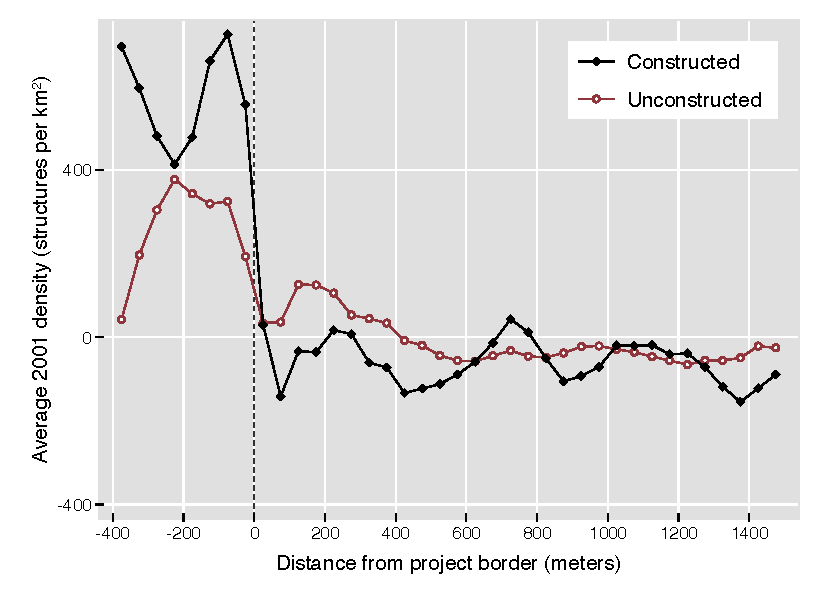
\includegraphics[width=\textwidth,trim={0.3cm .3cm 0.1cm 0cm}, clip=true]{figures/bblu_inf_fe_pre_means_4_2_30k.pdf}

        \end{subfigure}
        \begin{subfigure}[b]{0.48\textwidth}
                    \caption[Network2]%
            {{\footnotesize \textbf{Other} pre-period formal lat-lon fe }}   
            \label{fig:prefor}
            \centering
            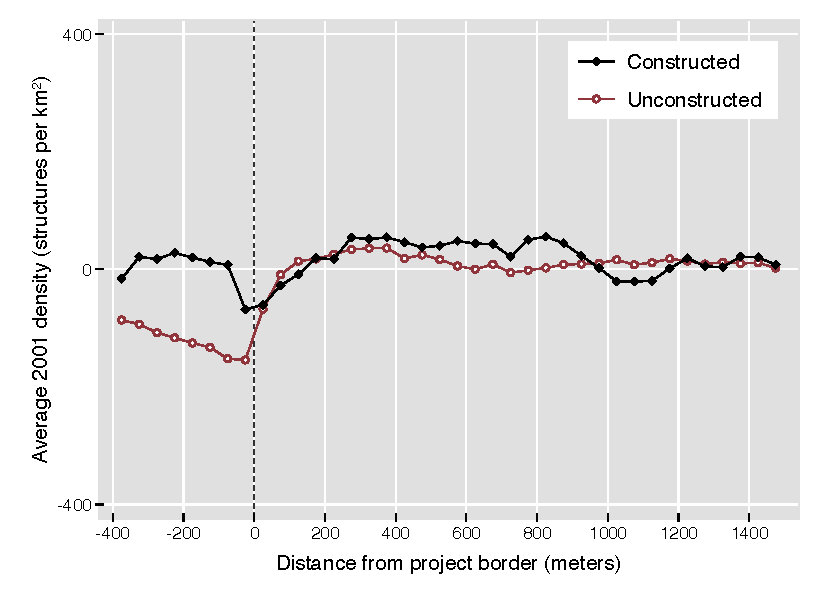
\includegraphics[width=\textwidth,trim={0.3cm .3cm 0.1cm 0cm}, clip=true]{figures/bblu_for_fe_pre_means_4_3_30k.pdf}

        \end{subfigure}
        \hfill
        \begin{subfigure}[b]{0.48\textwidth}  
                    \caption[]%
            {{\footnotesize \textbf{Other} pre-period informal lat-lon fe }}      
            \label{fig:preinf}
            \centering 
            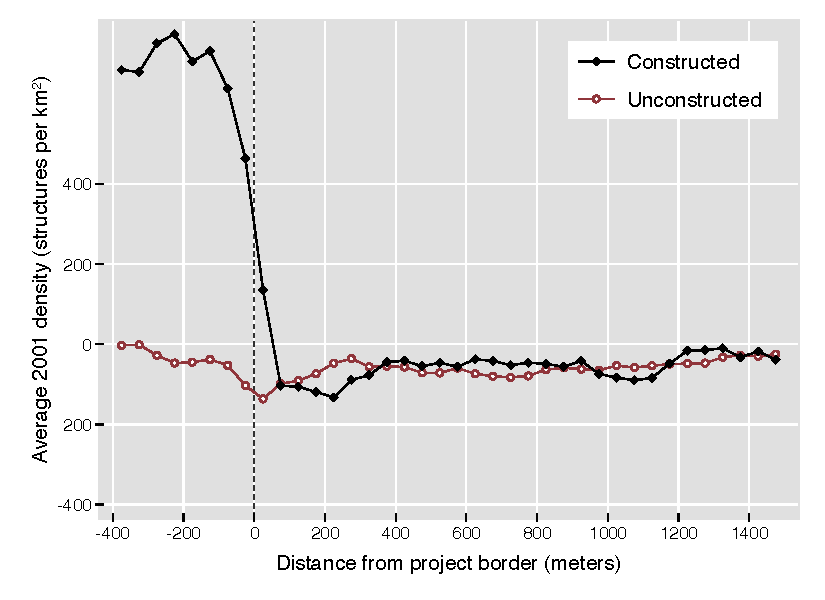
\includegraphics[width=\textwidth,trim={0.3cm .3cm 0.1cm 0cm}, clip=true]{figures/bblu_inf_fe_pre_means_4_3_30k.pdf}

        \end{subfigure}
\end{figure*}










\begin{figure*}
        \centering
   %     \caption[ Pre-Period Housing Densities in Constructed and Unconstructed Projects Areas ]
  %      {\small Pre-Period Densities} 
        %\vspace{2mm}
        \begin{subfigure}[b]{0.48\textwidth}
            \caption[Network2]%
            {{\footnotesize \textbf{All Projects} changes formal raw data}}    
            \label{fig:prefor}
            \centering
            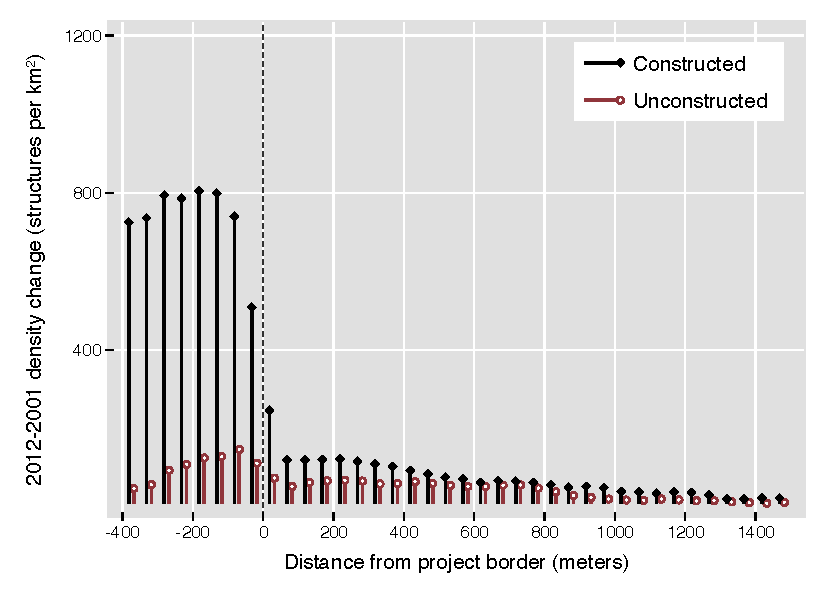
\includegraphics[width=\textwidth,trim={0.3cm .3cm 0.1cm 0cm}, clip=true]{figures/bblu_for_rawchanges_4_30k.pdf}

        \end{subfigure}
        \hfill
        \begin{subfigure}[b]{0.48\textwidth}  
                    \caption[]%
            {{\footnotesize \textbf{All Projects} changes informal  raw data}}      
            \label{fig:preinf}
            \centering 
            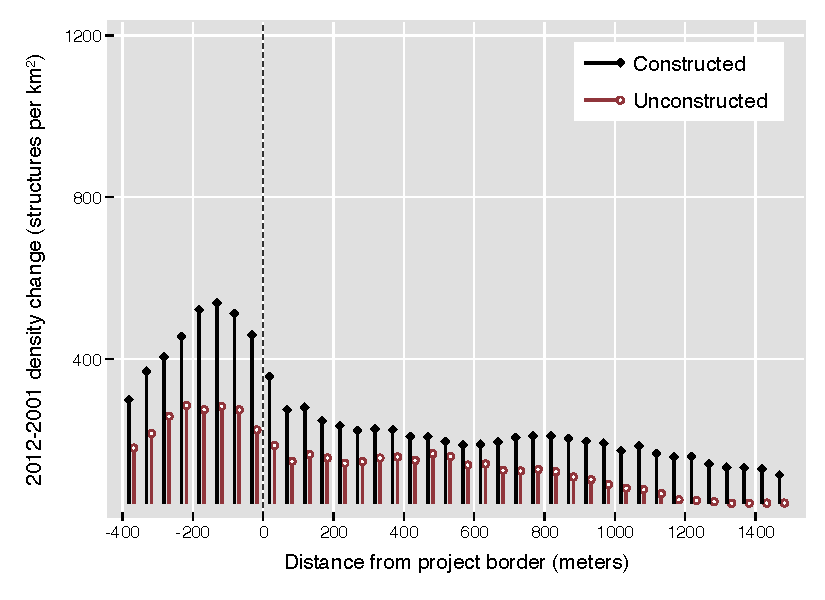
\includegraphics[width=\textwidth,trim={0.3cm .3cm 0.1cm 0cm}, clip=true]{figures/bblu_inf_rawchanges_4_30k.pdf}

        \end{subfigure}
        \begin{subfigure}[b]{0.48\textwidth}
                    \caption[Network2]%
            {{\footnotesize \textbf{Greenfield} changes formal  raw data}}    
            \label{fig:prefor}
            \centering
            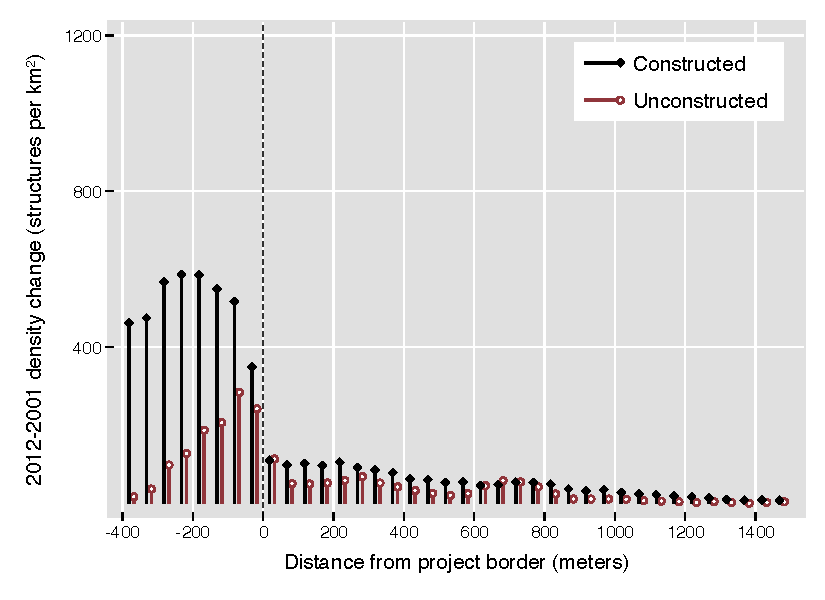
\includegraphics[width=\textwidth,trim={0.3cm .3cm 0.1cm 0cm}, clip=true]{figures/bblu_for_rawchanges_4_1_30k.pdf}

        \end{subfigure}
        \hfill
        \begin{subfigure}[b]{0.48\textwidth}  
                    \caption[]%
            {{\footnotesize \textbf{Greenfield} changes informal raw data }}     
            \label{fig:preinf}
            \centering 
            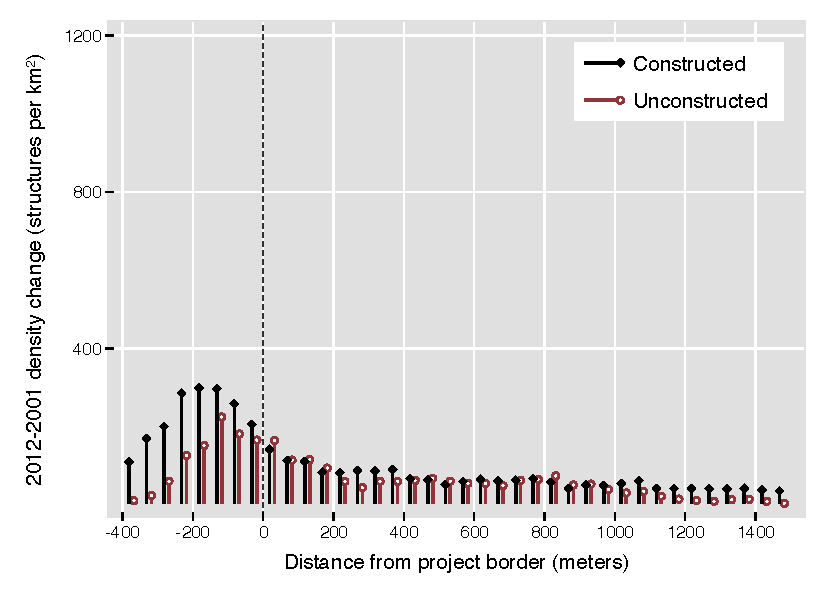
\includegraphics[width=\textwidth,trim={0.3cm .3cm 0.1cm 0cm}, clip=true]{figures/bblu_inf_rawchanges_4_1_30k.pdf}

        \end{subfigure}
        \begin{subfigure}[b]{0.48\textwidth}
                    \caption[Network2]%
            {{\footnotesize \textbf{In-Situ} changes formal raw data }}   
            \label{fig:prefor}
            \centering
            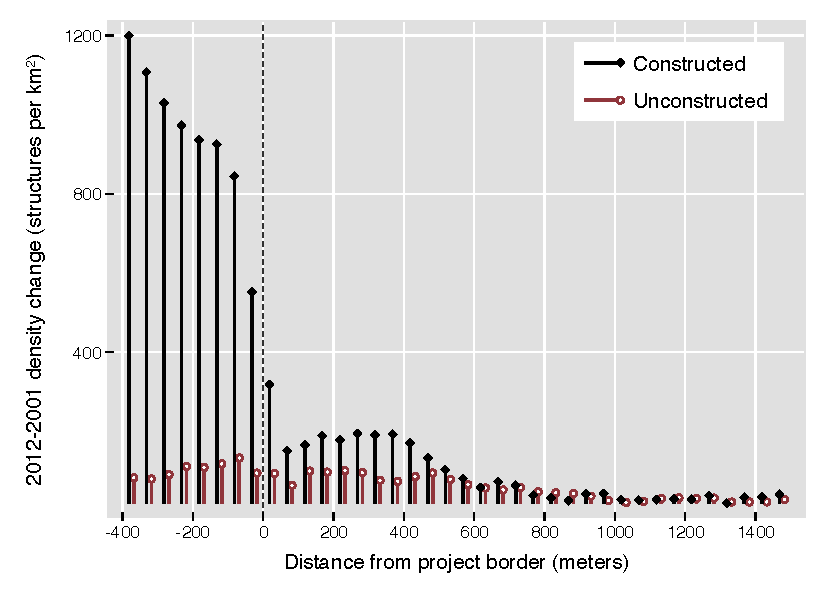
\includegraphics[width=\textwidth,trim={0.3cm .3cm 0.1cm 0cm}, clip=true]{figures/bblu_for_rawchanges_4_2_30k.pdf}

        \end{subfigure}
        \hfill
        \begin{subfigure}[b]{0.48\textwidth}  
                    \caption[]%
            {{\footnotesize \textbf{In-Situ} changes informal raw data }}     
            \label{fig:preinf}
            \centering 
            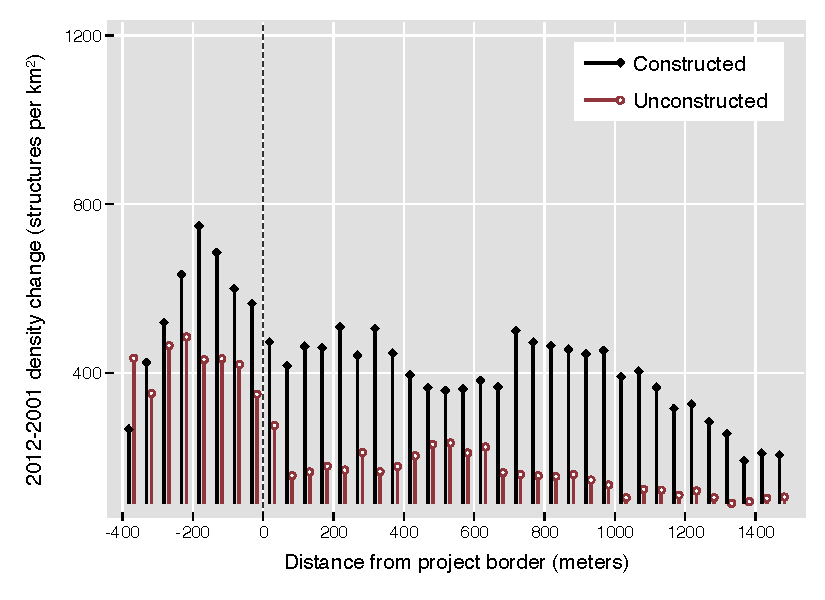
\includegraphics[width=\textwidth,trim={0.3cm .3cm 0.1cm 0cm}, clip=true]{figures/bblu_inf_rawchanges_4_2_30k.pdf}

        \end{subfigure}
        \begin{subfigure}[b]{0.48\textwidth}
                    \caption[Network2]%
            {{\footnotesize \textbf{Other} changes formal raw data}}   
            \label{fig:prefor}
            \centering
            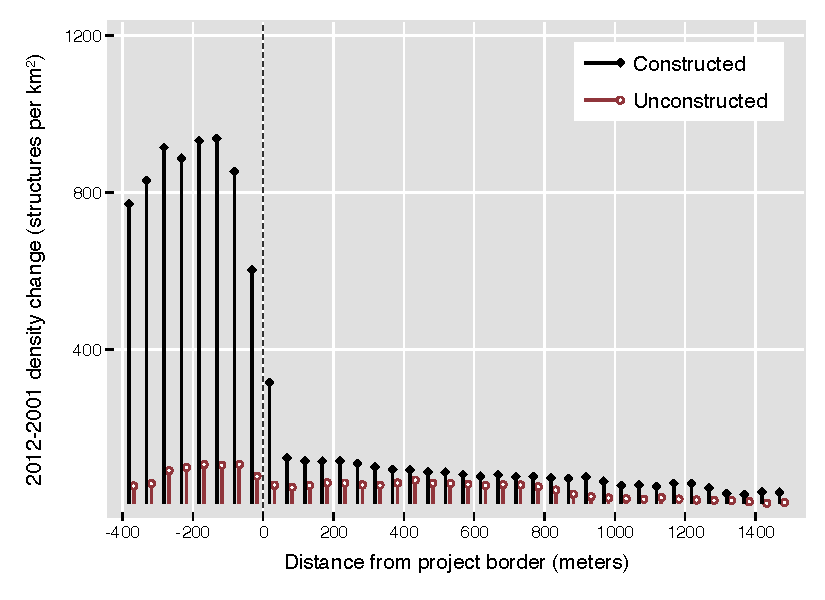
\includegraphics[width=\textwidth,trim={0.3cm .3cm 0.1cm 0cm}, clip=true]{figures/bblu_for_rawchanges_4_3_30k.pdf}

        \end{subfigure}
        \hfill
        \begin{subfigure}[b]{0.48\textwidth} 
                    \caption[]%
            {{\footnotesize \textbf{Other} changes informal  raw data}}      
            \label{fig:preinf} 
            \centering 
            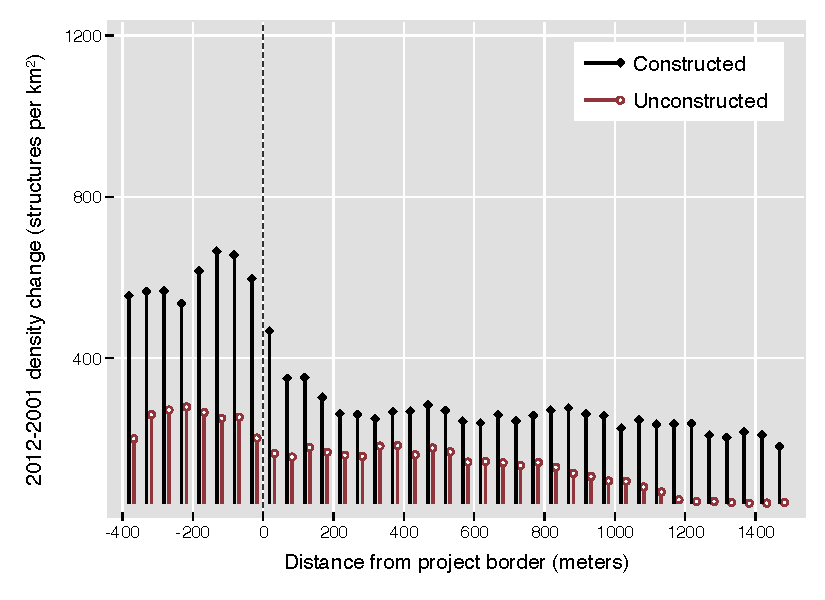
\includegraphics[width=\textwidth,trim={0.3cm .3cm 0.1cm 0cm}, clip=true]{figures/bblu_inf_rawchanges_4_3_30k.pdf}

        \end{subfigure}
\end{figure*}







\begin{table}
\caption{Building Density}
\begin{tabular}{lDDDDD}
\toprule
 & \small (1) & \small (2)  & \small (3) & \small (4) & \small (5) \\
 & Total & Formal  & Informal & Informal Bkyd. & Informal Non-Bkyd. \\ \midrule
\textbf{All Projects} \\inside project      &     679.071\textsuperscript{a}&     588.753\textsuperscript{a}&      90.319                   &     546.776\textsuperscript{a}&    -456.457\textsuperscript{a}\\
                    &   (139.895)                   &    (71.555)                   &   (114.372)                   &    (97.504)                   &    (88.617)                   \\[0.5em]
0-300m outside project &      81.944\textsuperscript{c}&      50.603\textsuperscript{b}&      31.341                   &      73.339\textsuperscript{b}&     -41.999                   \\
                    &    (46.400)                   &    (23.418)                   &    (41.379)                   &    (34.243)                   &    (32.359)                   \\[0.5em]
300-600m outside project &      -4.626                   &      16.885                   &     -21.511                   &       5.565                   &     -27.077                   \\
                    &    (29.510)                   &    (15.098)                   &    (26.968)                   &    (24.467)                   &    (18.853)                   \\[0.5em]
R$^2$               &       0.278                   &       0.251                   &       0.222                   &       0.235                   &       0.137                   \\

\midrule
\textbf{Greenfield} \\   inside project      &     202.124                   &     220.542                   &     -18.418                   &     100.816                   &    -119.234                   \\
                    &   (231.675)                   &   (141.954)                   &   (125.921)                   &   (137.676)                   &    (73.764)                   \\[0.01em]
0-300m outside project &    -101.751                   &     -28.602                   &     -73.149                   &     -78.024                   &       4.875                   \\
                    &    (76.515)                   &    (38.859)                   &    (57.073)                   &    (60.443)                   &    (47.802)                   \\[0.01em]
300-600m outside project&     -64.789\textsuperscript{c}&     -15.862                   &     -48.926\textsuperscript{c}&     -29.575                   &     -19.352                   \\
                    &    (33.609)                   &    (16.733)                   &    (25.433)                   &    (18.892)                   &    (20.372)                   \\[0.8em] 
\textbf{In-Situ Upgrading} \\   inside project      &     599.569                   &     821.733\textsuperscript{a}&    -222.164                   &     667.371\textsuperscript{b}&    -889.535\textsuperscript{a}\\
                    &   (377.899)                   &   (158.672)                   &   (285.666)                   &   (277.330)                   &   (258.069)                   \\[0.01em]
0-300m outside project &     158.197                   &      96.396                   &      61.801                   &     104.978                   &     -43.177                   \\
                    &   (176.693)                   &   (105.939)                   &   (116.646)                   &   (155.415)                   &   (116.730)                   \\[0.01em]
300-600m outside project &      82.268                   &      74.300                   &       7.967                   &      -5.156                   &      13.124                   \\
                    &   (108.679)                   &    (68.391)                   &    (81.768)                   &    (95.053)                   &    (85.593)                   \\[0.8em]
\textbf{Other} \\   inside project      &     963.847\textsuperscript{a}&     677.551\textsuperscript{a}&     286.297\textsuperscript{b}&     738.791\textsuperscript{a}&    -452.494\textsuperscript{a}\\
                    &   (168.333)                   &    (72.336)                   &   (142.792)                   &   (114.785)                   &   (105.179)                   \\[0.01em]
0-300m outside project &     101.629                   &      48.431\textsuperscript{b}&      53.199                   &      93.119\textsuperscript{b}&     -39.920                   \\
                    &    (69.177)                   &    (23.216)                   &    (62.855)                   &    (45.170)                   &    (39.931)                   \\[0.01em]
300-600m outside project &     -32.027                   &       2.226                   &     -34.253                   &       7.734                   &     -41.988\textsuperscript{b}\\
                    &    (43.203)                   &    (14.398)                   &    (41.794)                   &    (34.361)                   &    (20.161)                   \\[0.8em]
Mean Outcome 2001   &      379.90                   &      203.91                   &      175.98                   &       66.26                   &      109.72                   \\
Mean Outcome 2011   &      584.70                   &      281.66                   &      303.04                   &      192.77                   &      110.27                   \\
R$^2$               &       0.287                   &       0.253                   &       0.234                   &       0.238                   &       0.152                   \\
N                   &   2,721,910                   &   2,721,910                   &   2,721,910                   &   2,721,910                   &   2,721,910                   \\

\bottomrule
\end{tabular}
\end{table}





\begin{table}[h!] 
\caption{Effect of Housing Projects on Socio-demographics}
\label{table:sorting}
\small
\centering
%\caption{Census Composition Estimates }
\vspace{-2mm}
\begin{tabular}{lDDDDD}
\toprule
& \small (1) & \small (2) & \small (3) & \small (4)& \small (5)\\
& \small Age & \small P.O.B. not Gauteng & \small Unemployed & \small Years of Education & \small Monthly Income \\ \midrule 
\textbf{All Projects} \\inside project      &       0.112                   &      -0.029                   &      -0.008                   &       0.165                   &     333.092                   \\
                    &     (0.298)                   &     (0.021)                   &     (0.021)                   &     (0.158)                   &   (553.256)                   \\[0.5em]
0-300m outside project &       0.425                   &       0.021                   &       0.009                   &       0.078                   &     -78.108                   \\
                    &     (0.285)                   &     (0.016)                   &     (0.016)                   &     (0.115)                   &   (524.996)                   \\[0.5em]
300-600m outside project &       0.045                   &       0.011                   &       0.019                   &       0.095                   &      91.017                   \\
                    &     (0.304)                   &     (0.016)                   &     (0.016)                   &     (0.103)                   &   (459.385)                   \\[0.5em]
R$^2$               &       0.513                   &       0.614                   &       0.419                   &       0.584                   &       0.539                   \\

\midrule
\textbf{Greenfield} \\   inside project      &      -1.291\textsuperscript{c}&       0.024                   &       0.038                   &      -0.105                   &     801.640                   \\
                    &     (0.778)                   &     (0.040)                   &     (0.056)                   &     (0.399)                   &   (614.092)                   \\[0.01em]
0-300m outside project &      -0.418                   &       0.047                   &       0.033                   &       0.139                   &     616.062                   \\
                    &     (0.607)                   &     (0.031)                   &     (0.039)                   &     (0.259)                   &  (1089.422)                   \\[0.01em]
300-600m outside project&      -0.599                   &       0.014                   &       0.031                   &       0.645\textsuperscript{a}&      -7.217                   \\
                    &     (0.647)                   &     (0.029)                   &     (0.040)                   &     (0.233)                   &   (750.897)                   \\[0.8em] 
\textbf{In-Situ Upgrading} \\   inside project      &       0.512                   &      -0.057\textsuperscript{a}&      -0.053\textsuperscript{c}&       0.396                   &      96.742                   \\
                    &     (0.475)                   &     (0.021)                   &     (0.027)                   &     (0.298)                   &  (1224.985)                   \\[0.01em]
0-300m outside project &      -0.093                   &      -0.013                   &      -0.006                   &       0.321                   &     -52.987                   \\
                    &     (0.479)                   &     (0.024)                   &     (0.028)                   &     (0.222)                   &  (1027.733)                   \\[0.01em]
300-600m outside project &      -0.392                   &      -0.005                   &      -0.003                   &       0.091                   &    -464.643                   \\
                    &     (0.665)                   &     (0.024)                   &     (0.029)                   &     (0.207)                   &   (930.939)                   \\[0.8em]
\textbf{Other} \\   inside project      &      -0.027                   &       0.009                   &       0.000                   &       0.017                   &     268.658                   \\
                    &     (0.449)                   &     (0.031)                   &     (0.029)                   &     (0.211)                   &   (657.251)                   \\[0.01em]
0-300m outside project &       0.883\textsuperscript{c}&       0.036                   &       0.001                   &      -0.078                   &    -271.926                   \\
                    &     (0.456)                   &     (0.025)                   &     (0.024)                   &     (0.151)                   &   (742.485)                   \\[0.01em]
300-600m outside project &       0.446                   &       0.024                   &       0.023                   &      -0.099                   &     301.008                   \\
                    &     (0.438)                   &     (0.025)                   &     (0.020)                   &     (0.143)                   &   (672.828)                   \\[0.8em]
Mean Outcome 2001   &       27.31                   &        0.37                   &        0.47                   &        8.27                   &    2,480.46                   \\
Mean Outcome 2011   &       28.29                   &        0.43                   &        0.33                   &        9.68                   &    4,506.34                   \\
R$^2$               &       0.518                   &       0.622                   &       0.422                   &       0.587                   &       0.542                   \\
N                   &      12,733                   &      12,728                   &      12,725                   &      12,728                   &      12,724                   \\

\bottomrule
\multicolumn{6}{l}{\footnotesize Standard errors clustered at the project level in parenthesis. \textsuperscript{c} p$<$0.10, \textsuperscript{b} p$<$0.05, \textsuperscript{a} p$<$0.01  }\\
\multicolumn{6}{l}{\footnotesize P.O.B. means ``place of birth.''  Monthly income is in Rands.}
\end{tabular}
\end{table}








\begin{landscape}
{\footnotesize

\begin{table}[]
\small
\centering
\caption{Census Household-level Estimates }\label{table:censusestimates}
\vspace{-2mm}
\resizebox{.9\linewidth}{!}{
\begin{tabular}{lDDDDDDDD}
\toprule
 & \small (1) & \small (2)  & \small (3) & \small (4) & \small (5)  & \small (6)  & \small (7) & (8)\\
 & \small Flush Toilet & \small Water Indoors  & \small Electricity Cooking & \small Electricity Heating & \small Electricity Lighting  & \small Number of Rooms  & \small Household Size & Population Density\\ \midrule 
\textbf{All Projects} \\inside project      &       0.097                   &       0.182\textsuperscript{a}&       0.182\textsuperscript{a}&       0.163\textsuperscript{a}&       0.107                   &       0.069                   &       0.070                   &    -813.497                   \\
                    &     (0.069)                   &     (0.046)                   &     (0.064)                   &     (0.062)                   &     (0.066)                   &     (0.169)                   &     (0.079)                   &  (1228.688)                   \\[0.5em]
0-300m outside project &      -0.042                   &       0.015                   &      -0.015                   &      -0.003                   &      -0.025                   &      -0.092                   &      -0.094\textsuperscript{c}&     385.617                   \\
                    &     (0.036)                   &     (0.038)                   &     (0.034)                   &     (0.036)                   &     (0.032)                   &     (0.119)                   &     (0.054)                   &   (647.578)                   \\[0.5em]
300-600m outside project &      -0.033                   &       0.009                   &      -0.015                   &      -0.001                   &      -0.017                   &      -0.093                   &      -0.048                   &    -247.696                   \\
                    &     (0.027)                   &     (0.033)                   &     (0.027)                   &     (0.029)                   &     (0.026)                   &     (0.109)                   &     (0.052)                   &   (694.350)                   \\[0.5em]
R$^2$               &       0.402                   &       0.414                   &       0.491                   &       0.474                   &       0.442                   &       0.475                   &       0.496                   &       0.458                   \\

\midrule
\textbf{Greenfield} \\   inside project      &      -0.033                   &       0.131                   &       0.073                   &       0.035                   &       0.024                   &       0.251                   &       0.200                   &    3790.441\textsuperscript{c}\\
                    &     (0.131)                   &     (0.123)                   &     (0.111)                   &     (0.112)                   &     (0.126)                   &     (0.367)                   &     (0.209)                   &  (2196.802)                   \\[0.01em]
0-300m outside project &      -0.054                   &       0.077                   &       0.014                   &       0.036                   &      -0.030                   &       0.565\textsuperscript{c}&       0.257\textsuperscript{b}&    3716.468                   \\
                    &     (0.089)                   &     (0.091)                   &     (0.060)                   &     (0.069)                   &     (0.057)                   &     (0.287)                   &     (0.125)                   &  (2418.104)                   \\[0.01em]
300-600m outside project&       0.017                   &      -0.025                   &       0.086\textsuperscript{c}&       0.078                   &       0.096\textsuperscript{b}&       0.207                   &       0.126                   &    -466.573                   \\
                    &     (0.060)                   &     (0.076)                   &     (0.044)                   &     (0.059)                   &     (0.042)                   &     (0.195)                   &     (0.102)                   &  (1702.631)                   \\[0.8em] 
\textbf{In-Situ Upgrading} \\   inside project      &       0.320\textsuperscript{a}&       0.217\textsuperscript{b}&       0.347\textsuperscript{a}&       0.379\textsuperscript{a}&       0.220\textsuperscript{b}&       0.322                   &       0.169                   &   -3307.188                   \\
                    &     (0.111)                   &     (0.096)                   &     (0.090)                   &     (0.082)                   &     (0.095)                   &     (0.267)                   &     (0.128)                   &  (3071.103)                   \\[0.01em]
0-300m outside project &       0.018                   &       0.014                   &       0.069                   &       0.093                   &       0.026                   &      -0.250                   &      -0.012                   &    -919.031                   \\
                    &     (0.079)                   &     (0.079)                   &     (0.070)                   &     (0.077)                   &     (0.067)                   &     (0.274)                   &     (0.086)                   &  (1398.915)                   \\[0.01em]
300-600m outside project &      -0.007                   &       0.022                   &       0.051                   &       0.097                   &       0.002                   &      -0.234                   &      -0.083                   &    -269.849                   \\
                    &     (0.064)                   &     (0.074)                   &     (0.068)                   &     (0.072)                   &     (0.056)                   &     (0.301)                   &     (0.088)                   &  (1162.953)                   \\[0.8em]
\textbf{Other} \\   inside project      &      -0.078                   &       0.122\textsuperscript{b}&       0.062                   &       0.020                   &       0.019                   &      -0.302                   &      -0.093                   &    -585.210                   \\
                    &     (0.090)                   &     (0.059)                   &     (0.095)                   &     (0.091)                   &     (0.096)                   &     (0.235)                   &     (0.104)                   &  (1046.339)                   \\[0.01em]
0-300m outside project &      -0.073                   &       0.004                   &      -0.081\textsuperscript{c}&      -0.074\textsuperscript{c}&      -0.060                   &      -0.169                   &      -0.236\textsuperscript{a}&     -51.983                   \\
                    &     (0.045)                   &     (0.053)                   &     (0.045)                   &     (0.044)                   &     (0.043)                   &     (0.149)                   &     (0.078)                   &   (873.961)                   \\[0.01em]
300-600m outside project &      -0.062\textsuperscript{c}&       0.018                   &      -0.071\textsuperscript{c}&      -0.060\textsuperscript{c}&      -0.055                   &      -0.138                   &      -0.121                   &    -338.772                   \\
                    &     (0.033)                   &     (0.046)                   &     (0.036)                   &     (0.035)                   &     (0.035)                   &     (0.136)                   &     (0.076)                   &   (880.842)                   \\[0.8em]
Mean Outcome 2001   &        0.79                   &        0.35                   &        0.66                   &        0.62                   &        0.77                   &        3.30                   &        3.51                   &    8,566.83                   \\
Mean Outcome 2011   &        0.83                   &        0.54                   &        0.81                   &        0.72                   &        0.82                   &        3.56                   &        3.18                   &    9,823.82                   \\
R$^2$               &       0.414                   &       0.425                   &       0.500                   &       0.482                   &       0.450                   &       0.483                   &       0.502                   &       0.463                   \\
N                   &      12,732                   &      12,732                   &      12,732                   &      12,732                   &      12,732                   &      12,709                   &      12,730                   &      12,734                   \\

\bottomrule
\multicolumn{9}{l}{\footnotesize All regressions include 3km grid Fixed-Effects. Standard errors clustered at the project level in parenthesis. \textsuperscript{c} p$<$0.10,\textsuperscript{b} p$<$0.05,\textsuperscript{a} p$<$0.01 }
\end{tabular}
}
\end{table}

}
\end{landscape}




\begin{table}
\small
\centering
\caption{Triple Difference Estimates on Log-Prices}\label{table:priceDDD_het}
\vspace{-2mm}
\begin{tabular}{lCC}
\toprule
 & \small (1) & \small (2)  \\ \midrule 
 \textbf{All Projects} \\
 inside project      &       0.352                   &       0.357                   \\
                    &     (0.536)                   &     (0.536)                   \\[0.55em]
0-300m outside project &      -0.160                   &      -0.159                   \\
                    &     (0.173)                   &     (0.173)                   \\[0.5em]
300-600m outside project &      -0.062                   &      -0.060                   \\
                    &     (0.130)                   &     (0.130)                   \\[0.5em]
Lot Size Controls   &                               &  \checkmark                   \\
r2                  &        0.18                   &        0.18                   \\
N                   &      67,751                   &      67,751                   \\

 \midrule
\textbf{Greenfield} \\   inside project      &       0.200                   &       0.203                   \\
                    &     (0.475)                   &     (0.473)                   \\[0.01em]
0-300m outside project &       0.093                   &       0.092                   \\
                    &     (0.285)                   &     (0.285)                   \\[0.01em]
300-600m outside project&       0.048                   &       0.050                   \\
                    &     (0.277)                   &     (0.279)                   \\[0.8em]
\textbf{In-Situ Upgrading} \\   inside project      &       0.406                   &       0.423                   \\
                    &     (0.566)                   &     (0.571)                   \\[0.01em]
0-300m outside project &      -0.083                   &      -0.082                   \\
                    &     (0.401)                   &     (0.401)                   \\[0.01em]
300-600m outside project &      -0.155                   &      -0.155                   \\
                    &     (0.233)                   &     (0.234)                   \\[0.8em]
\textbf{Other} \\   inside project      &      -0.031                   &      -0.031                   \\
                    &     (0.581)                   &     (0.581)                   \\[0.01em]
0-300m outside project &      -0.232                   &      -0.230                   \\
                    &     (0.210)                   &     (0.210)                   \\[0.01em]
300-600m outside project &      -0.083                   &      -0.080                   \\
                    &     (0.169)                   &     (0.170)                   \\[0.8em]
Lot Size Controls   &                               &  \checkmark                   \\
r2                  &        0.21                   &        0.21                   \\
N                   &      67,751                   &      67,751                   \\

\bottomrule
\multicolumn{3}{l}{\footnotesize Standard errors clustered at the project level in parenthesis.} \\
\multicolumn{3}{l}{ \textsuperscript{c} p$<$0.10,\textsuperscript{b} p$<$0.05,\textsuperscript{a} p$<$0.01 }
\end{tabular}
\end{table} 

\begin{figure}
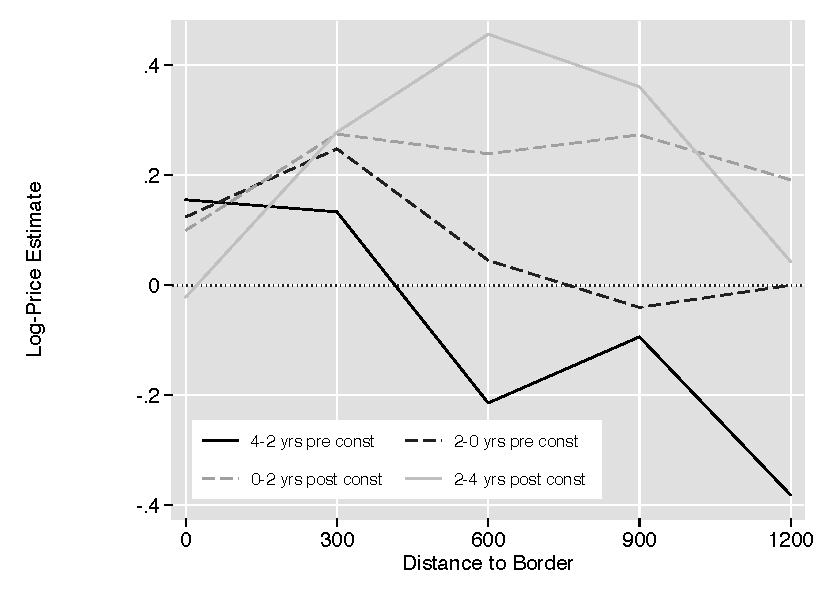
\includegraphics{figures/price_to_event_30.pdf}
\end{figure}


\end{document}


